\subsection{Forward Commitments}

\begin{remark} \hlt{No-Arbitrage Principle}\\
There should be no risk-less profit to be gained by a combination of forward contract and other assets.
\begin{enumerate}[label=\roman*.]
\setlength{\itemsep}{0pt}
\item Transaction costs are zero (market frictions are nil)
\item Replicating instruments are identifiable and investable
\item Short selling is allowed with full use of proceeds
\item Borrowing and lending are available at a known risk-free rate
\end{enumerate}
\end{remark}

\begin{remark} \hlt{Carry Arbitrage Model}\\
No-arbitrage approach where the underlying instrument is either bought or sold along with establishing a forward position. Models account for costs to carry the underlying asset, such as financing costs plus storage and insurance costs. Model also adjusts for carry benefits such as dividends and interests received.
\end{remark}

\begin{flushleft}
Characteristics of Futures and Forward Contracts
\begin{tabularx}{\textwidth}{X|X}
\hline
\rowcolor{gray!30}
Futures & Forwards \\
\hline
Exchange-Traded & Negotiated between contract and counterparties\\
\hline
Standardised dates and deliverables & Customised dates and deliverables\\
\hline
Trades guaranteed by clearinghouse & Trades subjected to counterparty risk\\
\hline
Initial value $=0$ & Initial value $=0$ (typically, but not required)\\
\hline
Initial margin deposit required. Margin account adjusted for G\&L daily. If daily losses caused by margin balance drops below maintenance margin, additional funds to be deposited or position will be closed.
&
Margin requirements may be specified by counterparties.\\
\hline
Daily settlement marks contract price equal to market price and contract value $=0$ &
Contract may outline settlement schedule. Forward may accumulate or los value between settlement periods or until maturity.\\
\hline
\end{tabularx}
\end{flushleft}

\begin{remark} \hlt{Convergence Property of Futures and Forwards}\\
At expiration time $T$, both the forward price $F_T$ and futures price $f_t$ are equivalent to spot price $S_T$.
\begin{equation}
F_T = f_T = S_T \nonumber
\end{equation}
\end{remark}

\begin{figure}[H]
\centering
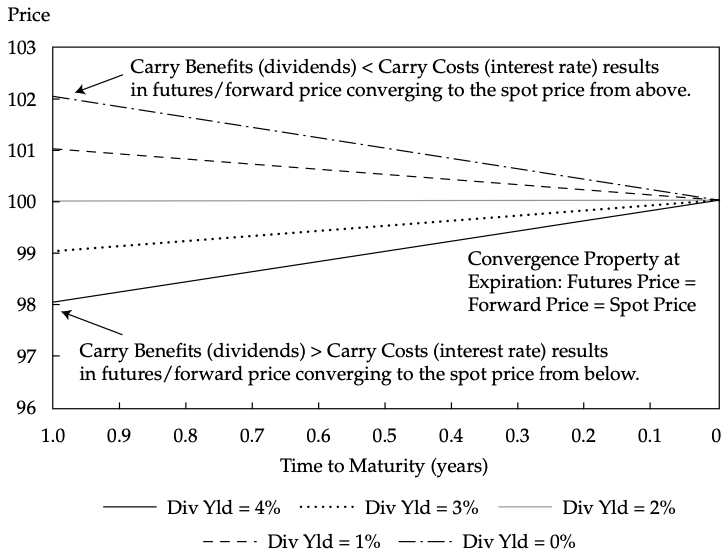
\includegraphics[scale=0.4]{/derivatives/convgprop}
\caption{Convergence property of forward price to spot price}
\end{figure}

\begin{definition} \hlt{Price of Forward Contract}
\begin{equation}
F_0 = S_0 \times (1+r_f)^T \nonumber
\end{equation}
where $F_0$ is forward price, $S_0$ is spot price at inception of contract, $r_f$ is annual risk free rate.
\end{definition}

\begin{flushleft}
Cash flows from long underlying and short forward
\begin{tabularx}{\textwidth}{X|X|X}
\hline
\rowcolor{gray!30}
& Time $0$ & Time $T$ \\
\hline
\textbf{Borrow funds to long asset} & & \\
Underlying & $-S_0$ (purchase) & $+S_T$ (sale) \\
Borrowed Funds & $+S_0$ (inflow) & $-FV(S_0)$ (repayment) \\
Net Cash Flow & $-S_0 + S_0 = 0$ & $+S_T - FV(S_0)$ \\
\textbf{Short Forward} & & \\
Short Forward & $V_0 = 0$ & $V_T = F_0 - S_T$ \\
\textbf{Overall} & & \\
& $+S_0 - S_0 + V_0 = 0$ & $+S_T - FV(S_0) + V_T = 0$\\
& & $+S_T - FV(S_0) + (F_0 - S_T) = 0$\\
& & $+F_0 - FV(S_0) = 0$\\
\textbf{Net} & $0$ & $F_0 = FV(S_0)$\\
\hline 
\end{tabularx}
\end{flushleft}

\begin{remark} \hlt{Carry Arbitrage and Reverse Carry Arbitrage}\\
Buy underpriced assets and sell overpriced assets, take opposite positions in spot and forward markets.\\
In the case that forward is overpriced, to engage in carry arbitrage
\begin{enumerate}[label=\roman*.]
\setlength{\itemsep}{0pt}
\item Sell forward contract on underlying
\item Borrow funds to purchase the underlying
\item Purchase the underlying
\end{enumerate}
In the case that the forward is underpriced, to engage in reverse carry arbitrage
In the case that forward is overpriced, to engage in carry arbitrage
\begin{enumerate}[label=\roman*.]
\setlength{\itemsep}{0pt}
\item Buy forward contract on underlying
\item Short the underlying
\item Lend the short sale proceeds
\end{enumerate}
\end{remark}

\begin{remark} \hlt{Value of Forward Contract}
\begin{equation}
V_t = PV(F_t - F_0) = \frac{F_t - F_0}{(1+r)^{T-t}} = S_t - \frac{F_0}{(1-r)^{T-t}} \nonumber
\end{equation}
where $V_t$ is value of forward contract at time $t$, $PV$ is present value, $F_t$ is price of forward contract at time $t$.\\
Basis of $T = t/365$ is used for Equity Forward Contracts.\\
If the forward contract has cost of carry $CC_0$ and cost of benefit $CB_0$, then the price of contract is
\begin{equation}
F_0 = FV(S_0 + CC_0 - CB_0) \nonumber
\end{equation}
The value of the forward contract will use the adjusted price of contract as input.\\
$FV$ will use exponential in the case of continuous compounding.
\end{remark}

\begin{remark} \hlt{Forward Rate Agreements (FRA)}\\
An OTC forward contract where the underlying is an interest rate on a deposit.\\
The fixed-rate payer is long FRA, the fixed-rate receiver is short FRA.\\
Long position will profit when market reference rate (MRR) rises above rate in FRA.\\
FRAs are settled in cash for the difference between fixed interest payment established on initiation date and a floating interest payment established on FRA expiration date.\\
FRAs are identified by $h \times m$, and payoff is based on spot $m$-day MRR observed in $h$-days from FRA initiation.
\end{remark}

\begin{figure}[H]
\centering
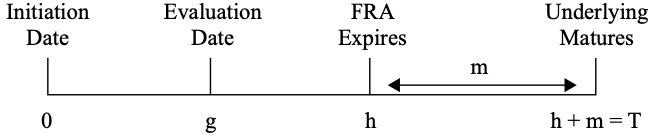
\includegraphics[scale=0.35]{/derivatives/hmfra}
\caption{A $h \times m$ FRA}
\end{figure}

\begin{remark} \hlt{FRA Settlement Terminologies}\\
Either by 'advanced set, settled in arrears' or 'advanced set, advanced settled' (typically for FRAs).
\begin{enumerate}[label=\roman*.]
\setlength{\itemsep}{0pt}
\item Advanced set: reference interest rate is set at the time the money is deposited.
\item Settled in Arrears: interest payment is made at time $h+m$, the maturity of the instrument.
\item Advanced Settle: settlement made at time $h$.
\end{enumerate}
\end{remark}

\begin{remark} \hlt{Add-On Basis of FRA}\\
FRA uses add-on basis for MRR, where the terminal amount is expressed as
\begin{equation}
TA = NA \times (1 + L_m t_m) \nonumber
\end{equation}
where $NA$ is notional amount, $L_m$ is MRR spot rate (set at time $t=0$) for $m$-day deposit, $t_m = m/360$ is accrual period as a fraction for $m$-day deposit.
Interest paid is then
\begin{equation}
TA - NA = NA \times (L_m t_m) \nonumber
\end{equation}
\end{remark}

\begin{method} \hlt{Pricing of FRAs}
\begin{enumerate}[label=\roman*.]
\setlength{\itemsep}{0pt}
\item Long position incurs gain when rates rise, incurs loss when rates decrease. Vice versa for short position.
\item FRA price $FRA_0$ is implied forward rate for the period beginning when FRA expires to underlying loan maturity. Hence two spot rates are required to determine the implied forward rate.
\item Although interest on underlying loan won't be paid until end of the loan, payoff on FRA will occur at expiration of FRA 9advanced settled), hence payoff on FRA is present value of interest savings on loan.
\end{enumerate}
The annualised FRA is then
\begin{equation}
FRA_0 = \left(\frac{1 + L_T t_T}{1 + L_h t_h} - 1 \right)/t_m \nonumber
\end{equation}
\end{method}

\begin{method} \hlt{Valuation of FRAs}\\
The value of FRA comes from interest savings on a loan to be made at settlement date, and when this value is to be received (at end of the loan), then computed to present value.\\
Let fixed-rate at initiation be $FRA_0$, and rate of FRA at time $g$ be $FRA_g$. The value of long FRA is then
\begin{equation}
V_g = NA \times \frac{FRA_g - FRA_0}{1 + D_{(T-g)} t_{(T_g)}} \nonumber
\end{equation}
\end{method}

\begin{figure}[H]
\centering
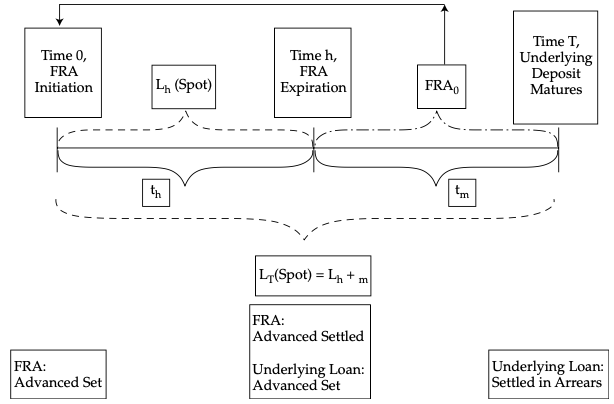
\includegraphics[scale=0.5]{/derivatives/pricefra}
\caption{FRA rates based on spot MRR}
\end{figure}

\begin{remark} \hlt{Characteristics of Fixed-Income Forwards}\\
Fixed-income forwards have to adjust for accrued interest in valuation.\\
In addition, fixed-income forwards may have more than one bond that can be delivered by seller. As bonds trade at different prices based on maturity and stated coupon, a conversion factor $CF$ has to be applied to make all deliverable bonds approximately equal in price.\\
Third, when multiple bonds can be delivered for forward, a cheapest-to-deliver bond emerges after adjusting for the conversion factor.
\end{remark}

\begin{figure}[H]
\centering
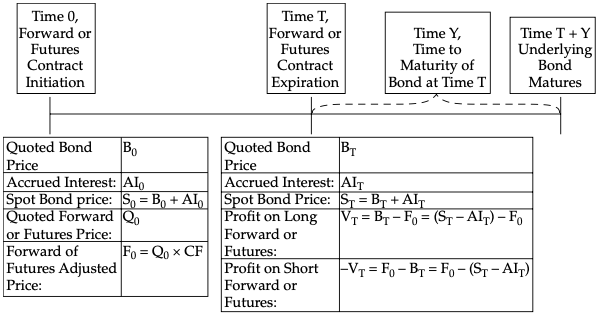
\includegraphics[scale=0.5]{/derivatives/bondfuttime}
\caption{Timeline for bond futures and forwards}
\end{figure}

\begin{method} \hlt{Pricing of Fixed-Income Forwards}\\
Let accrued interest be $AI$, number of accrued days since last coupon payment be $NAD$, number of total days in coupon payment period be $NTD$, annual coupon amount be $C$, number of coupon payments per year be $n$.
\begin{equation}
AI = \frac{NAD}{NTD} \times \frac{C}{n} \nonumber
\end{equation}
The fixed-income forwards prices is then
\begin{align}
F_0 &= FV(B_0 - AI_0 - PVCI) \nonumber \\
Q_0 &= \frac{F_0}{CF} \nonumber
\end{align}
where $B_0$ is full bond price at initiation, $AI_0$ is accused interest at initiation, $PVCI = CB_0$ is present value of all coupon interest paid over forward contract horizon from $t = 0$ to $t = T$, $Q_0$ is quoted futures price, $CF$ is the conversion factor.
\end{method}

\begin{method} \hlt{Value of Fixed-Income Forwards}\\
Value of forward contract at time $t$ is
\begin{equation}
V_t = PV(F_t - F_0) \nonumber
\end{equation}
\end{method}

\begin{remark} \hlt{Futures Contracts}\\
Requires mark-to-market, where margin balance of the futures account is adjusted each day to account for change in value of contract from previous trading day, based on settlement price.\\
Priced similar to forwards, except with adjustment for mark-to-market, as forwards do not accumulate value changes over the term of the contract.
\begin{equation}
\text{Value of futures} = \text{Current futures price} - \text{previous mark-to-market price} \nonumber
\end{equation}
\end{remark}